\subsubsection{RLPx Transport Protocol}
\label{sec:rlpx-transport-protocol}

The aim of this protocol is to provide a generalized mean to build arbitrary
authenticated and encrypted protocols. The protocols built on top of this
framework are known as subprotocols. Everyone can create a new subprotocol by
simply selecting $3$ ASCII characters to uniquely identify the protocol and by
defining a list of packet types and the expected structure of their content,
which will be encoded with the RLP algorithm.

\begin{figure}
  \begin{center}
    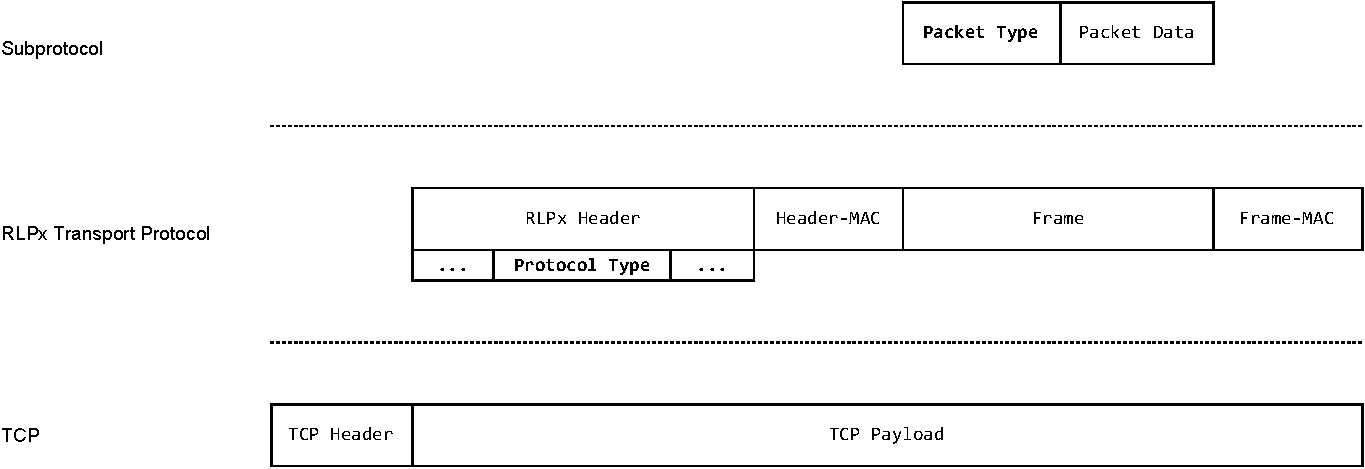
\includegraphics[width=\textwidth]{./res/img/rlpx-transport}
    \caption{Relationship between TCP, RLPx and the subprotocols}
    \label{fig:rlpx-transport}
  \end{center}
\end{figure}

The relationship between TCP, RLPx and the subprotocol packets is depicted
in~\autoref{fig:rlpx-transport}\footnote{For the sake of simplicity, here we
report only single-framed RLPx packets, but we redirect the interested reader to
the official documentation~\cite{rlpx} to get details about multi-framed
packets.}. The RLPx transport protocol packets are sent as payload in a TCP
packet. If we do not consider the MAC codes used to encrypt the information,
these packets consist of two fields:
\begin{itemize}
  \item a header, which specifies information such as the size of the frame and
  the subprotocol that will be used
  \item the frame, which is the packet of the subprotocol.
\end{itemize}

In turn the subprotocol packet contains a code that uniquely identify the
message type (packet-type) and its content (packet-data), that is specific to
the subprotocol. The content of this packet is serialized using the RLP
algorithm.

When two peers establish a connection with the RLPx transport protocol, they
perform a two-way handshake:
\begin{enumerate}
  \item encoding handshake, used to exchange a cryptographic secret\footnote{It
  is beyond the scope of this report to describe the exact procedure. For
  further details, we refer to the official documentation~\cite{rlpx} and to the
  Go Ethereum implementation
  \url{https://github.com/ethereum/go-ethereum/blob/master/p2p/rlpx.go}.}
  that is used to encrypt and authenticate the subsequent RLPx messages between
  them
  \item protocol handshake, in which the peers exchange and agree on the
  subprotocols and versions that both support (from now these pairs will be
  referred as \emph{capabilities}).
  %    send to the other one a \texttt{Hello}
  %    message, that contain the list of supported capabilities. Each one
  %    independently compute the list of common capabilities and sort it according
  %    to the lexicographic order. Since each protocol have a predefined amount
  %    of reserved message types, it is possible to build a data-structure to get
  %    from the packet-type the protocol-type. We show how it works with the mean
  %    of an easy example. Let's suppose that the peers have only the three protocols
\end{enumerate}

To perform the protocol handshake, and in general to establish and keep the
connection at this layer, the special subprotocol \devpp{} Wire
Protocol~\cite{devp2pwire} is involved. This subprotocol does not have an
identifier and reserves 16 message-types although only 4 are implemented. The
\verb+Hello+ (Handshake) message is used for the protocol handshake. This
message specifies, among others, the protocol version, the capabilities, the
port on which the client listens and the node ID. The \verb+Disconnect+ message
notifies the receiver that the sender is going to disconnect itself. The
disconnect message can specify optionally an integer that encodes a
reason\footnote{We refer to the \devpp{} specification~\cite{devp2pwire} for a
complete list of reason codes}. The \verb+Ping+ and \verb+Pong+ messages are
used to check whether the counterpart is still on-line or not.

After the protocol handshake, both peers know the shared capabilities. Since
each protocol have a predefined amount of reserved message types, sorting them
lexicographically it is possible to build a data-structure to retrieve the
protocol-type from the packet-type. We show how it works by means of an easy
example shown in~\autoref{table:capabilities}. Let's suppose that the peers
share the capabilities (expressed as tuples $\langle$subprotocol,
version$\rangle$) $\langle$abc, 4$\rangle$, $\langle$abc, 5$\rangle$ and
$\langle$zzz, 2$\rangle$ and that the capabilities reserve $9$, $11$ and $5$
message types respectively. The first row of the table represents the first $16$
message types reserved by the RLPx transport protocol. Then, if one of the peers
receives the message of type \texttt{0x1C}, it can determine that the message
should be interpreted as a message of type \texttt{0x01} of the capability
$\langle$abc, 5$\rangle$.

\begin{table}
  \begin{center}
    \begin{tabular}{c | c | c }
      Capability & Reserved IDs & Effective Packet Types\\
      \hline
      - & \texttt{[0x0, 0x10]} & \texttt{[0x0, 0x10]} \\
      $\langle$abc, 4$\rangle$ & \texttt{[0x0, 0x8]} & \texttt{[0x11, 0x1A]}  \\
      $\langle$abc, 5$\rangle$ & \texttt{[0x0, 0xA]} & \texttt{[0x1B, 0x26]}  \\
      $\langle$zzz, 2$\rangle$ & \texttt{[0x0, 0x4]}  & \texttt{[0x27, 0x3C]} \\
    \end{tabular}
    \caption{Example of data-structure built after the protocol handshake}
    \label{table:capabilities}
  \end{center}
\end{table}

We notice that, although the RLPx Header (\autoref{fig:rlpx-transport}) contains
a field to specify the protocol type, it is not used by the implementations of
Ethereum (at least geth and ethereumj\footnote{Since all the implementations
should be interoperable, it means that all the implementations do not use this
field or they deal with the case in which it is not used.}). If it would be the
case it would be sufficient to use the protocol-type in the RLPx header to
identify uniquely a protocol. The reason probably lies in the fact that \devpp{}
protocol do not have an identifier.
